\section{Sistema A – Controlo de Iluminação Interior}

Com um nível de luz entre 0 e 200 o LED encontra-se desligado.


\begin{figure}[H]
    \centering
    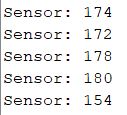
\includegraphics[scale=1.1]{images/testes/SisA_SerialMonitor0FF_original.png}
    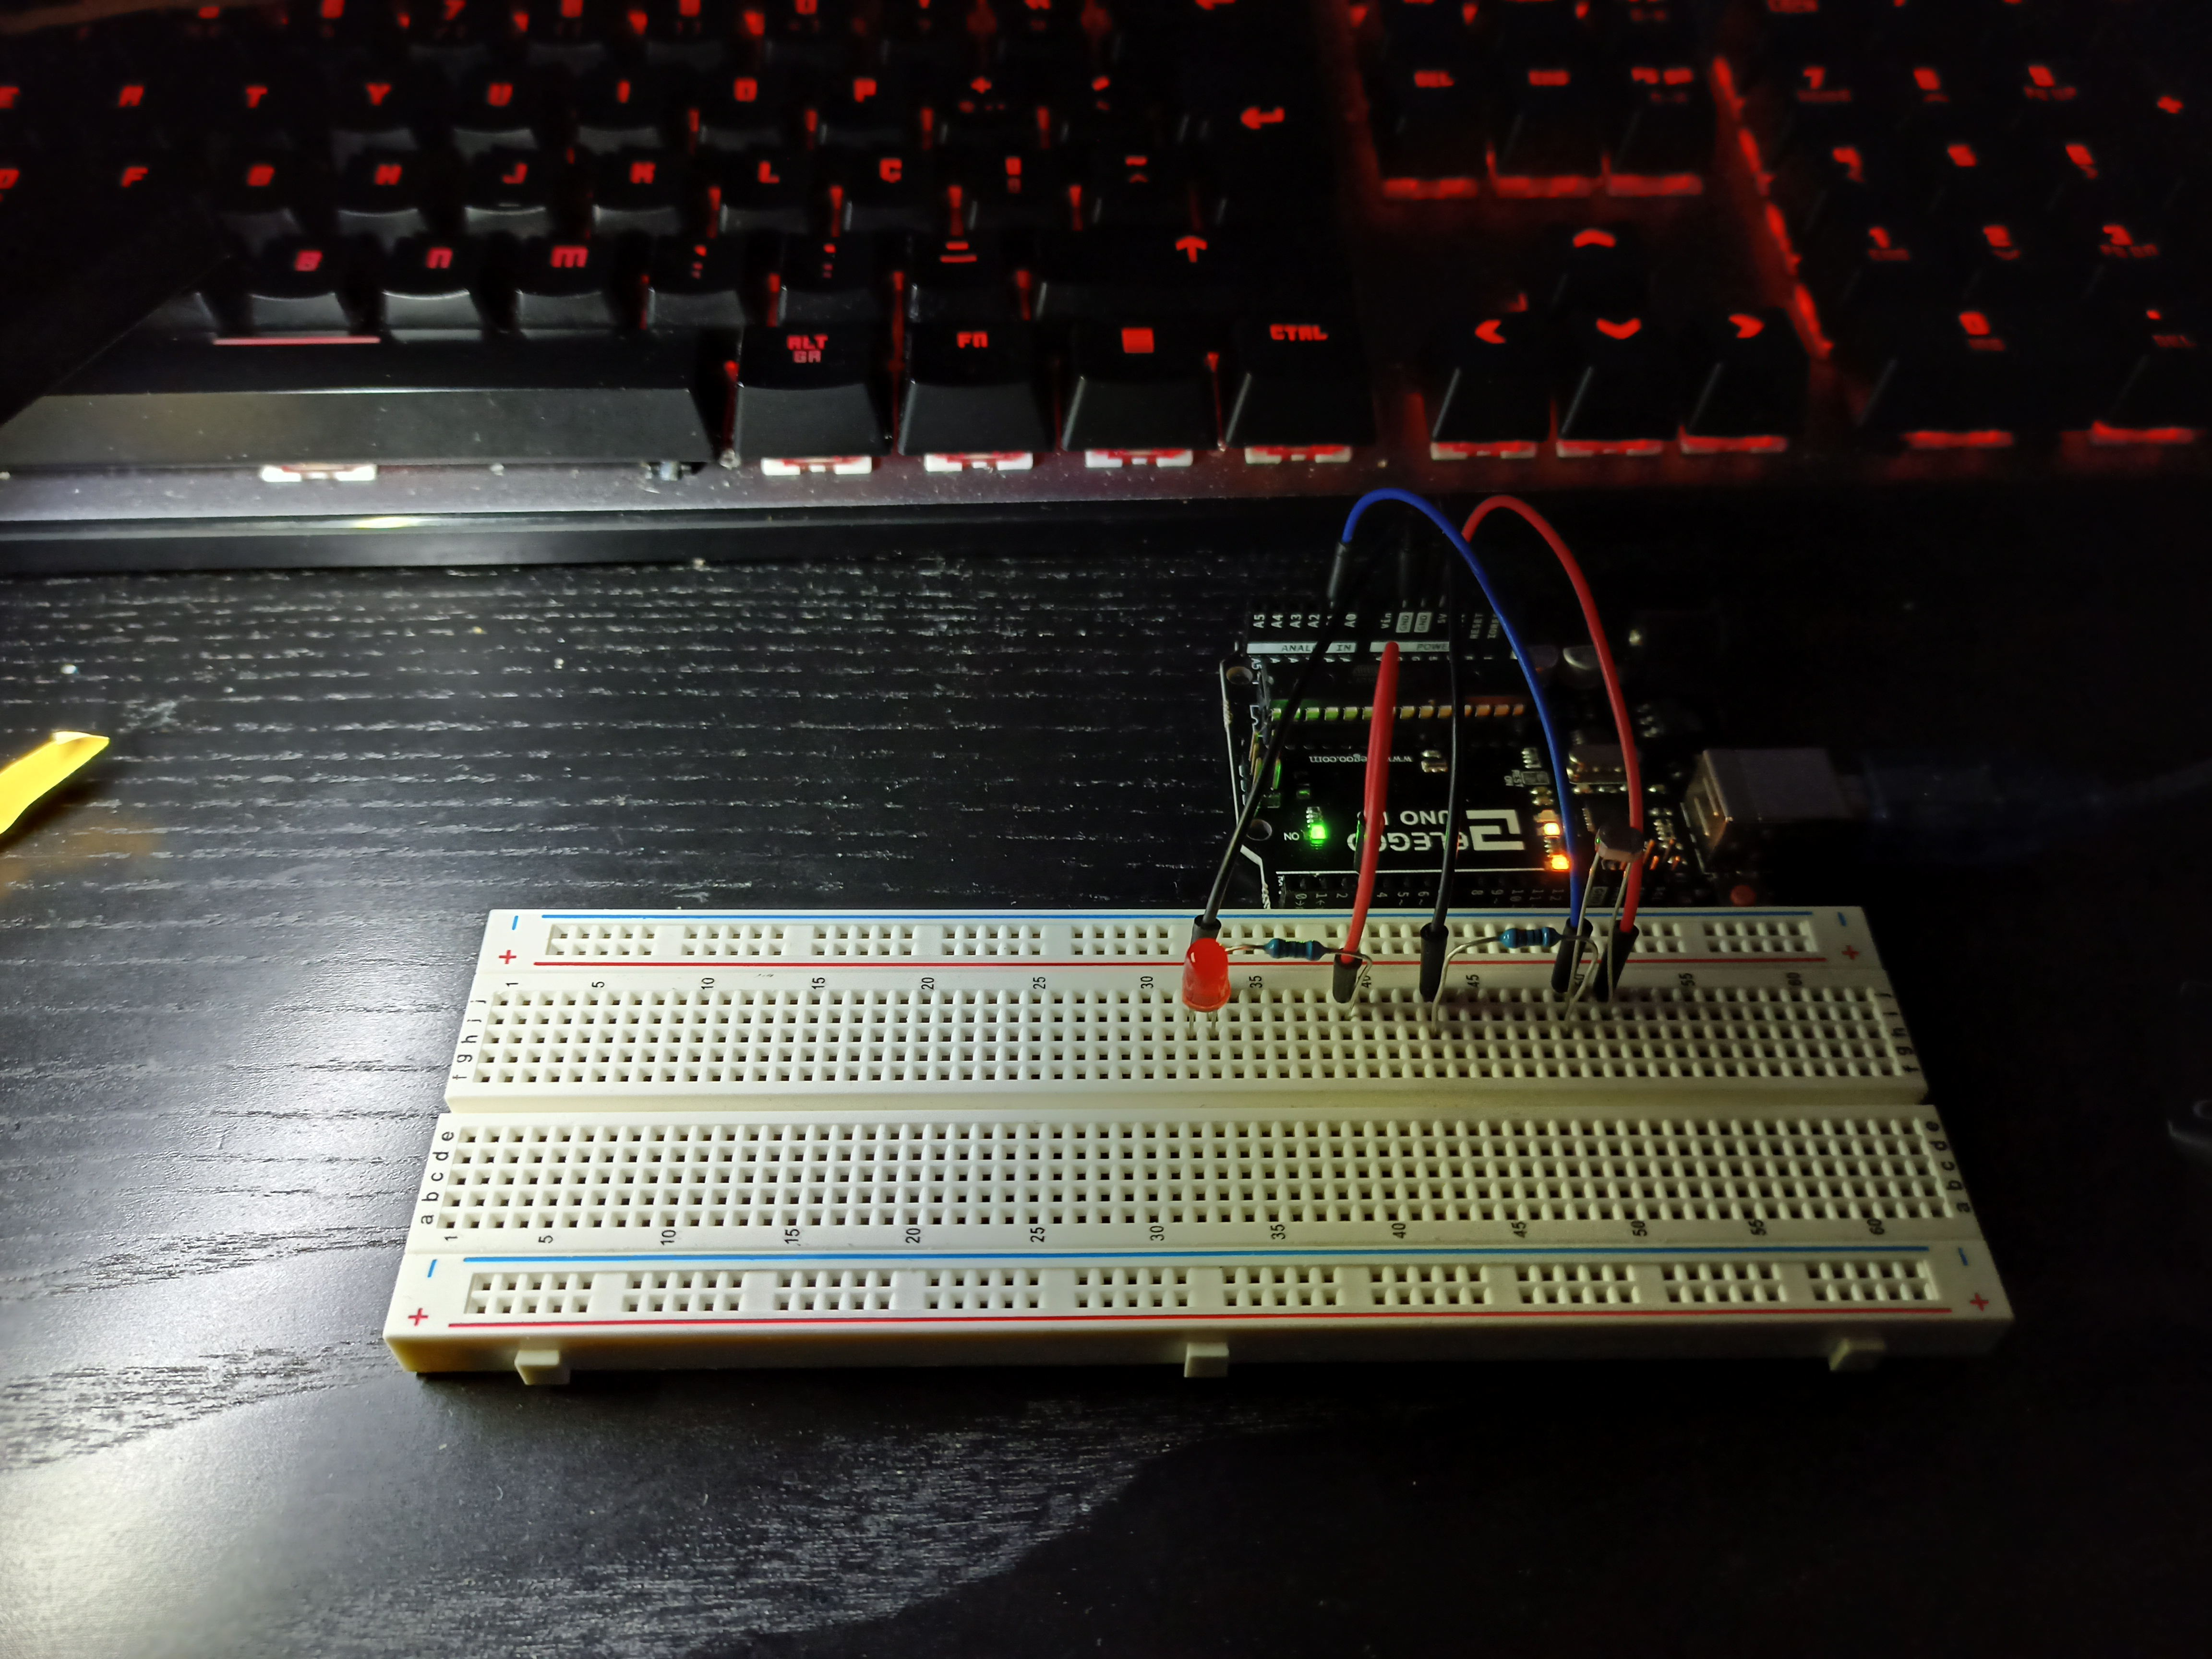
\includegraphics[scale=0.03]{images/testes/sisA_Off.jpg}
    \selectlanguage{portuguese}\caption{LED desligado no nivel inicial}
\end{figure}


Com um nível de luz entre 200 e 500 o LED encontra-se ligado com um valor de 64.

\begin{figure}[H]
    \centering
    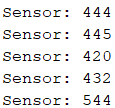
\includegraphics[scale=1.1]{images/testes/sisA_SerialMonitor1_original.png}
    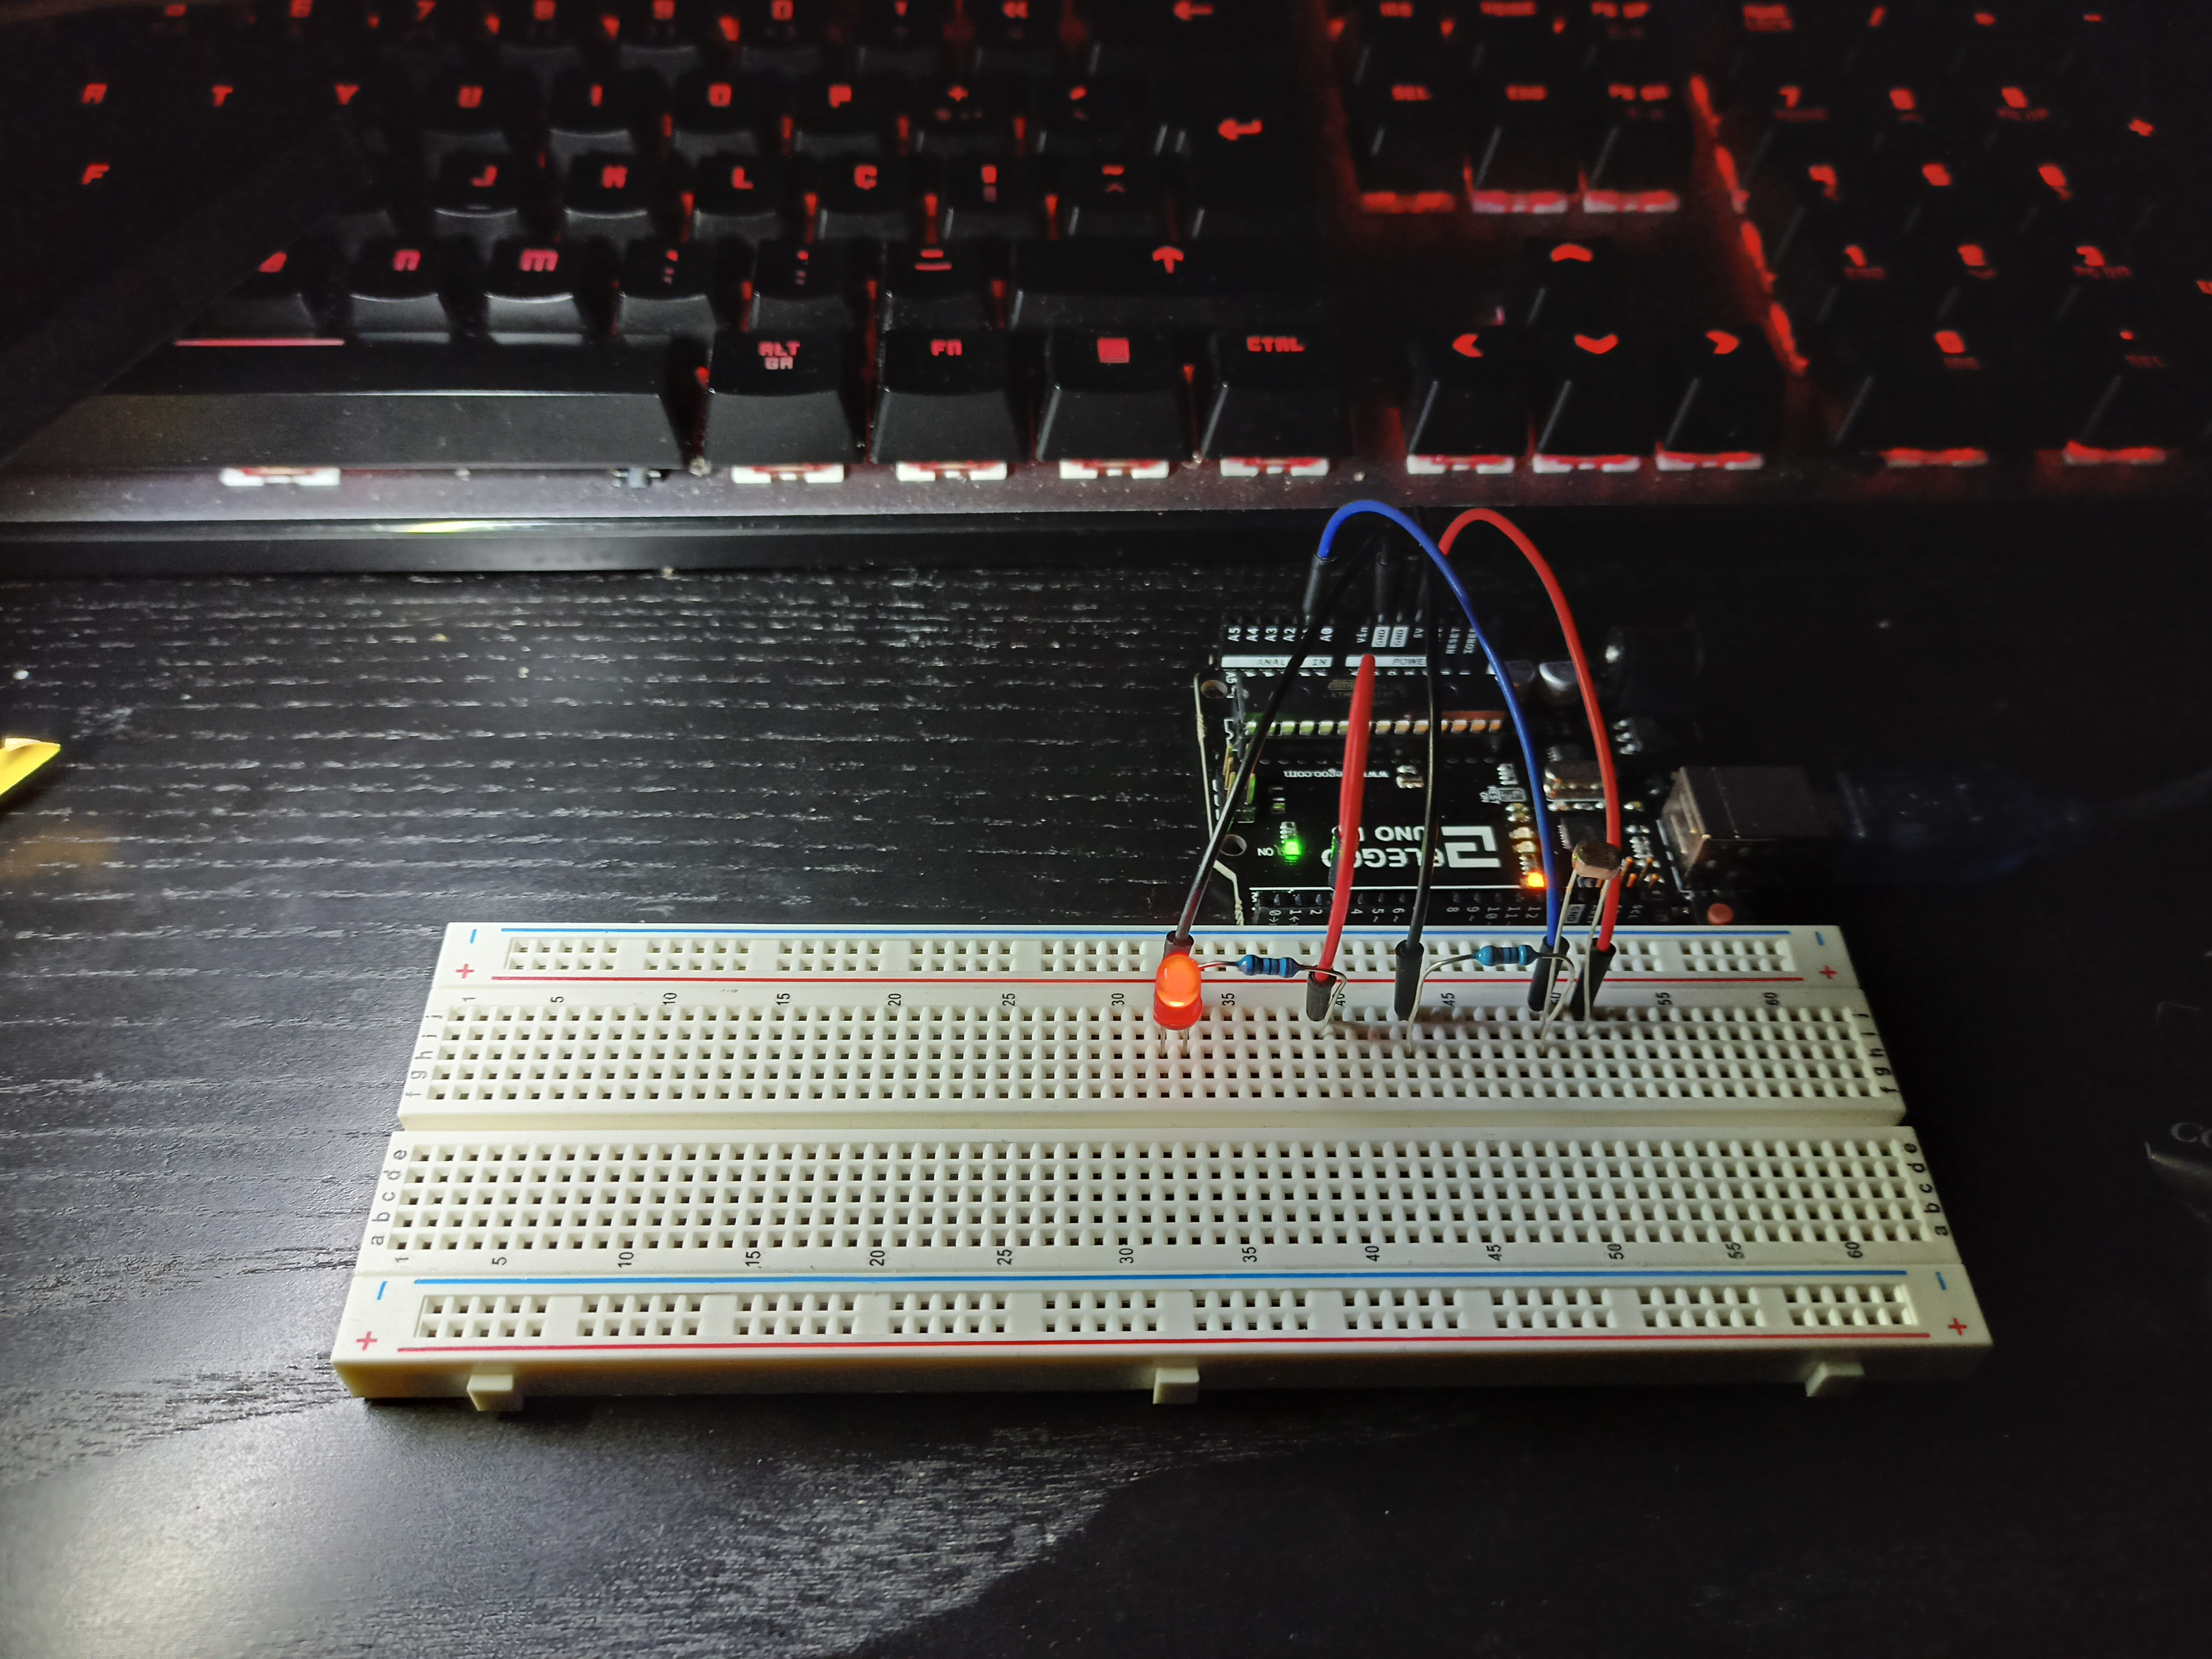
\includegraphics[scale=0.03]{images/testes/sisA_1.jpg}
    \selectlanguage{portuguese}\caption{LED ligado no nivel 1}
\end{figure}

Com um nível de luz entre 500 e 800 o LED encontra-se ligado com um valor de 128.

\begin{figure}[H]
    \centering
    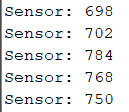
\includegraphics[scale=1.1]{images/testes/sisA_SerialMonitor2_original.png}
    \includegraphics[scale=0.03]{images/testes/sisA_2.jpg}
    \selectlanguage{portuguese}\caption{LED ligado no nivel 2}
\end{figure}

Com um nível de luz entre luz superior a 800 o LED encontra-se ligado com a potência máxima disponível.

\begin{figure}[H]
    \centering
    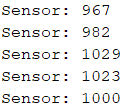
\includegraphics[scale=1.1]{images/testes/sisA_SerialMonitor3_original.png}
    \includegraphics[scale=0.03]{images/testes/sisA_3.jpg}
    \selectlanguage{portuguese}\caption{LED ligado no nivel máximo}
\end{figure}